\PageHeading{10}{案例C · 真实模型朋友圈}{聚焦一个可验证卖点，完整保留口径与适用条件}
\ModeLive
\begin{note}\small
\Lead{任务与过程}\quad 开学季面向大学新生，门店朋友圈渠道；真实调用模型策划，手动收敛为重量单卖点并保存大纲v2，确认后完成正文、独立审稿及必要修订，再生成竖形卡片。
\end{note}
\begin{minipage}[t]{.46\linewidth}\vspace{0pt}\centering
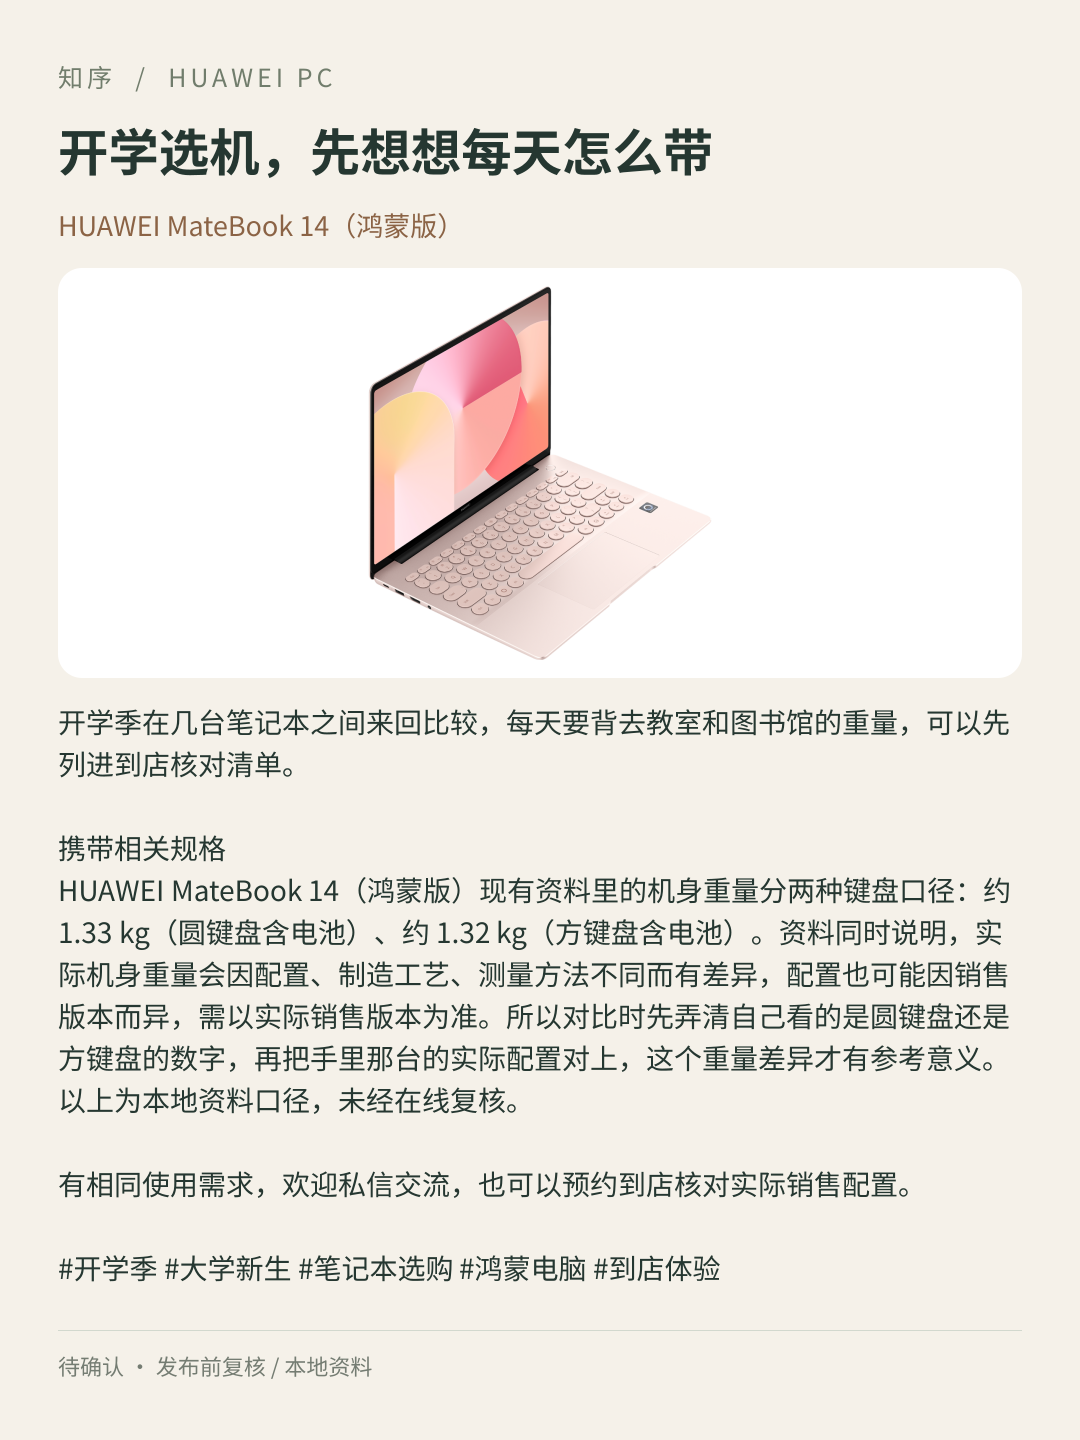
\includegraphics[height=112mm,width=\linewidth,keepaspectratio]{case-c-1.png}
\ImgCap{实际1080$\times$1440 PNG。页脚保留“待确认／本地资料”，与本地规则演示分开标记。}
\end{minipage}\hfill
\begin{minipage}[t]{.50\linewidth}\vspace{0pt}
\Lead{可确认的运行事实}\par
\begin{itemize}
\item 不是静态Mock：已调用配置的模型服务，并完成独立审稿调用。
\item 大纲v2的标题、段落、事实引用和配图由后端固定。
\item 只围绕重量，不扩展价格、性能或个人使用体验。
\item PNG与ZIP实际生成，较长条件采用竖形模板完整呈现。
\end{itemize}
\begin{attention}\small
\Lead{审核结果}\quad needs\_attention。证据来自本地快照，尚未经ima在线复核；不能据此声称产品信息为最新或已经通过正式发布审核。
\end{attention}
\end{minipage}
\Sub{真实模型正文原样节选}
\begin{excerpt}\small
\Lead{\CaseCTitle}\par
\CaseCFirst\par
\Lead{行动引导}\quad \CaseCCTA
\end{excerpt}
\Lead{质量观察}\quad 正文保留圆/方键盘两种条件、“约”的口径及配置、工艺、测量方法差异，主动说明本地资料未经在线复核。这里的证据只支持该次样例，不外推总体事实准确率。
\SourceNote{已有真实运行结果output/live-workflow，case-c.json保存去原始全文后的说明数据；本轮仅引用已有成品，没有新增模型调用。}
